\documentclass[11pt,a4paper,openany]{report}
\usepackage[T1]{fontenc}
\usepackage[utf8]{inputenc}
\usepackage{lmodern}
\usepackage{microtype}
\usepackage{amsmath,amssymb,amsthm,mathtools,bm}
\usepackage{booktabs,array,longtable,tabularx}
\usepackage{xcolor}
\usepackage[margin=24mm,headheight=23pt]{geometry}
\usepackage{enumitem}
\usepackage{fancyhdr}
\usepackage{fancyvrb}
\usepackage{graphicx}
\usepackage{url}
\usepackage{xurl}
\usepackage{hyperref}

\definecolor{finblue}{HTML}{1F5A99}
\definecolor{fingreen}{HTML}{19733A}
\definecolor{finorange}{HTML}{D55E00}
\definecolor{finred}{HTML}{A61B1B}
\definecolor{finviolet}{HTML}{6A3D9A}

\hypersetup{
  unicode=true,
  colorlinks=true,
  linkcolor=finblue,
  citecolor=fingreen,
  urlcolor=finblue,
  pdftitle={FIN Programs 101--112: Fractional Limits, Source Tests, and Operational Completion},
  pdfauthor={Krzysztof Żuchowski},
  pdfsubject={Schur nonclosure, graphon and fractional limits, adaptive dynamics, operational models, exponent source},
  pdfkeywords={FIN, fractional operator, Schur complement, graphon, stable process, information geometry, process tensor}
}

\pagestyle{fancy}
\fancyhf{}
\fancyhead[L]{\small FIN Programs 101--112}
\fancyhead[R]{\small Release 10.11}
\fancyfoot[C]{\thepage}
\setlength{\parindent}{0pt}
\setlength{\parskip}{0.55em}
\setlist{nosep,leftmargin=2em}
\setcounter{tocdepth}{2}
\setcounter{secnumdepth}{3}
\emergencystretch=3em

\newcommand{\one}{\bm 1}
\newcommand{\C}{\mathbb C}
\newcommand{\R}{\mathbb R}
\newcommand{\Z}{\mathbb Z}
\newcommand{\statusProven}{\textcolor{fingreen}{[Proven]}}
\newcommand{\statusComputer}{\textcolor{fingreen}{[Proven, computer-assisted]}}
\newcommand{\statusStrong}{\textcolor{finblue}{[Strong evidence]}}
\newcommand{\statusModerate}{\textcolor{finviolet}{[Moderate evidence]}}
\newcommand{\statusConditional}{\textcolor{finorange}{[Conditional]}}
\newcommand{\statusRefuted}{\textcolor{finred}{[Refuted]}}
\newcommand{\statusOpen}{\textcolor{finviolet}{[Open]}}

\begin{document}
\hypersetup{pageanchor=false}
\begin{titlepage}
\centering
\vspace*{9mm}
{\Large\bfseries FIN Research Monograph --- Release 10.11\par}
\vspace{11mm}
{\Huge\bfseries FIN Programs 101--112\par}
\vspace{6mm}
{\Large Fractional Limits, Source Tests,\\
and Operational Completion\par}
\vspace{17mm}
{\Large Krzysztof \.Zuchowski\par}
\vspace{2mm}
{\normalsize Independent Researcher --- Fractal Information Theory Project\par}
\vspace{2mm}
{\normalsize ORCID: \href{https://orcid.org/0009-0002-0909-3613}{0009-0002-0909-3613}\par}
\vspace{10mm}
{\large 27 July 2026\par}
{\normalsize Publication --- Preprint; record version 1.0.0\par}
\vfill
\begin{minipage}{0.88\textwidth}
\small
\textbf{Scope.} Twelve executed studies of independent strict-kernel
certification, graphon/local/fractional continuum limits, long-range
propagation, adaptive information geometry, inverse variational sources,
selector boundaries, preregistration, apparatus memory, and the conditional
source skeleton for the exponent \(9/5\).

\medskip
\textbf{Central result.} The infinite strict lattice is a symmetric
fractional generator of order \(4/5\), while a local Laplacian requires an
additional singular localization and clock scaling.  The identity
\(4\ln2\mapsto2^{-4/5}\mapsto d^{-9/5}\) is exact but remains conditional on
an unsourced fivefold quotient and damping coupling.

\medskip
\textbf{Guardrail.} No strict selector, physical-unit source, Lorentz closure,
legacy role transfer, completed legacy--strict bridge, role-bearing
\(L_{\mathrm{total}}\), or external physical validation is claimed.

\medskip
\textbf{License.} Creative Commons Attribution 4.0 International (CC BY 4.0).
\end{minipage}
\vfill
\end{titlepage}
\hypersetup{pageanchor=true}

\pagenumbering{roman}
\chapter*{Publication statement}
\addcontentsline{toc}{chapter}{Publication statement}
This release reports Programs 101--112 and recommends Programs 113--124.
Theorem-level statements, computer-assisted certificates, numerical evidence,
conditioned operational models, failed inferences, and open obligations are
labeled separately.

\tableofcontents
\clearpage
\pagenumbering{arabic}

\section{Confidence convention}

Claims are labeled as proven, computer-assisted, strong evidence, conditional, negative, or open. The precise meanings are stated again in Section 2.

\section{Abstract}

This monograph executes twelve research programs on the strict FIN kernel, its continuum limits, adaptive dynamics, operational interpretation, and the unresolved source of its compression exponent. The strict working profile is

\[
k(d)=\frac{|\cos(\omega d+\phi)|}{1+d^\eta},
\qquad
(\omega,\phi,\eta)=
\left(\frac{743}{4000},\frac{13}{80},\frac95\right).
\]

An independent directed-interval calculation proves that the normalized infinite strict lattice is not closed, even up to scalar normalization, under alternating-site Schur reduction. The separation margin is \(0.1495869758\) at mass \(1/4\), and a partitioned interval certificate remains positive for every mass in \([0.01,2]\). A 243-point perturbation audit is also positive, although it is explicitly not promoted to a continuous multi-parameter theorem.

The continuum analysis distinguishes three inequivalent limits. Regular coordinate rescaling converges in operator norm to a bounded convolution graphon. A local Laplacian appears only after an additional singular localization and an \(\epsilon^{-2}\) clock rescaling. The unscaled infinite lattice instead has the fractional small-wave-number law

\[
1-\widehat p(q)\sim C|q|^{4/5},
\]

with fitted exponent \(0.7983228\) and predicted Abelian constant \(C=1.1474680\). Its heat semigroup consequently has a one-big-jump far-tail law rather than an exponential propagation cone.

A Fisher--Shahshahani adaptive flow is constructed on the kernel-shell probability simplex and is proved to dissipate a declared information functional. It does not select the strict FIN profile. A six-feature inverse variational search can force stationarity at one graph size, but produces two nonunique saddles, fails transfer to a held-out graph size, and is more description-heavy than the four strict parameters.

The most compact exponent-source candidate found in this round is the exact conditional chain

\[
\alpha_{\rm geo}=4\ln2,\qquad
r_5=e^{-\alpha_{\rm geo}/5}=2^{-4/5},
\qquad
C(2d)=r_5C(d)
\Longrightarrow
C(d)\propto d^{-4/5}.
\]

Multiplying a legacy \(d^{-1}\) envelope then produces \(d^{-9/5}\). This is an exact compatibility theorem, not a strict source theorem: no current artifact derives the fivefold quotient, its non-target-coded coupling to damping, or a target-independent \(\beta\)/\allowbreak{}length standard. No new signed chiral source is found, QW-2191 remains open, and no physical theory is claimed.

\par\medskip\hrule\medskip

\chapter{Part I --- Scope, status language, and mathematical core}

\section{Research question}

Programs 101--112 ask five narrow questions.

\begin{enumerate}
\item 
Does the previously observed strict-kernel Schur nonclosure survive an independent arithmetic method and a nontrivial mass interval?

\item 
Which continuum operator is generated by each admissible scaling?

\item 
Does the strict long-range tail force fractional propagation?

\item 
Can an information-geometric adaptive law or a compact variational source derive the strict profile?

\item 
Can the recurring exponent \(9/5\) be generated from already present FIN constants without silently inserting the target?

\end{enumerate}

These questions do not authorize a generic reopening of closed legacy-to-strict, selector, role-transfer, or full-Lagrangian lanes.

\section{Status language}

Every material statement is assigned one of the following statuses.

\begin{itemize}
\item 
\textbf{Proven:} an analytic derivation is given from stated hypotheses.

\item 
\textbf{Proven, computer-assisted:} directed numerical enclosures and analytic remainder bounds jointly establish the claim.

\item 
\textbf{Strong evidence:} a robust numerical result supports, but does not by itself prove, an analytic claim.

\item 
\textbf{Conditional:} the conclusion is rigorous after adding explicitly named premises that FIN does not yet source.

\item 
\textbf{Negative result:} a declared finite candidate class fails its stated acceptance tests.

\item 
\textbf{Open:} the required source, theorem, or calibrated data are absent.

\end{itemize}

\section{Kernel split and ontology guardrails}

The primary object in this monograph is the completed strict working kernel

\[
K_{\rm strict}(d)
=
\frac{\cos(\omega d+\phi)}{1+\beta d^\eta}.
\]

The legacy kernel

\[
K_{\rm legacy}(d)
=
\alpha_{\rm geo}
\frac{\cos(\omega_{\rm L}d+\phi_{\rm L})}
{1+\beta_{\rm tors}d}
\]

is retained only as an intermediate bridge kernel. It is not a co-equal final kernel and is not silently substituted for the strict profile. The tail comparison in Program 112 is therefore a conditional completion calculation, not a completion certificate and not a legacy physical-role transfer.

The repository ontology is also preserved: the nadsoliton is primordial fractal information in a solitonic state. No lower informational layer is introduced. Mathematical operators used to represent information are not automatically identified with physical matter, clocks, apparatuses, or observers.

\section{Minimal operator used in the calculations}

On the infinite lattice, define

\[
a_d=
\frac{|\cos(\omega d+\phi)|}{1+d^\eta},
\qquad
Z=2\sum_{d\ge1}a_d,
\qquad
p_{\pm d}=\frac{a_d}{Z}.
\]

The normalized convolution operator is

\[
(Pf)(x)=\sum_{d\ne0}p_d f(x+d),
\]

and its positive generator is

\[
A_m=mI+I-P,\qquad m>0.
\]

The corresponding wave and diffusion families are

\[
U_t=e^{-itA_m},
\qquad
P_t=e^{-tA_m}.
\]

They share a generator, but they are not the same physical dynamics. A physical use requires a state, preparation, clock, instrument, environment, apparatus, record, and dimensional calibration.

\par\medskip\hrule\medskip

\chapter{Part II --- Programs 101--104: independent certification and continuum limits}

\section{Program 101 --- Independent directed-interval nonclosure certificate}

\subsection{Objective}

Recompute the strict Schur obstruction without reusing the floating-point summation engine of Program 91.

\subsection{Exact inputs and tail}

The calculation uses exact rational inputs

\[
\omega=\frac{743}{4000},\qquad
\phi=\frac{13}{80},\qquad
\eta=\frac95
\]

inside 50-decimal directed interval arithmetic. The first \(D=20\,000\) terms are enclosed term by term. Since

\[
0\le a_d\le d^{-9/5},
\]

the omitted two-sided normalization tail satisfies

\[
T_D
\le
2\sum_{d>D}d^{-9/5}
\le
\frac{2D^{-4/5}}{4/5}
=0.0009059745795971189.
\]

The directed partial normalization interval collapses at the printed precision to

\[
Z_D\in
[1.967128237564778,\;1.967128237564778].
\]

Adding the signed numerator tail and the nonnegative normalization tail gives

\[
\widehat p(\pi)
\in[-0.3447351882,-0.3436558012],
\]

\[
\widehat p(\pi/2)
\in[-0.1603026372,-0.1593081528].
\]

\subsection{Scale-invariant obstruction}

For alternating-site elimination, the retained precision symbol is the harmonic mean of the two aliased fine symbols. A scalar field or operator normalization cannot change a ratio of two spectral values. At \(m=1/4\) the native ratio is enclosed by

\[
R_{\rm native}\in
[0.1567658391,\;0.1568720170],
\]

whereas the Schur-retained ratio is

\[
R_{\rm Schur}\in
[0.3064589929,\;0.3067033963].
\]

Thus

\[
\inf R_{\rm Schur}-\sup R_{\rm native}
=0.1495869759>0.
\]

\textbf{Result 101.1 --- \statusComputer{}.} The fixed-mass normalized infinite strict lattice is not closed, even up to scalar normalization, under one alternating-site Schur step.

This conclusion is limited to the declared coarse map and fixed profile. It does not exclude parameter running, new counterterms, or a different renormalization transformation.

\begin{figure}[htbp]
\centering
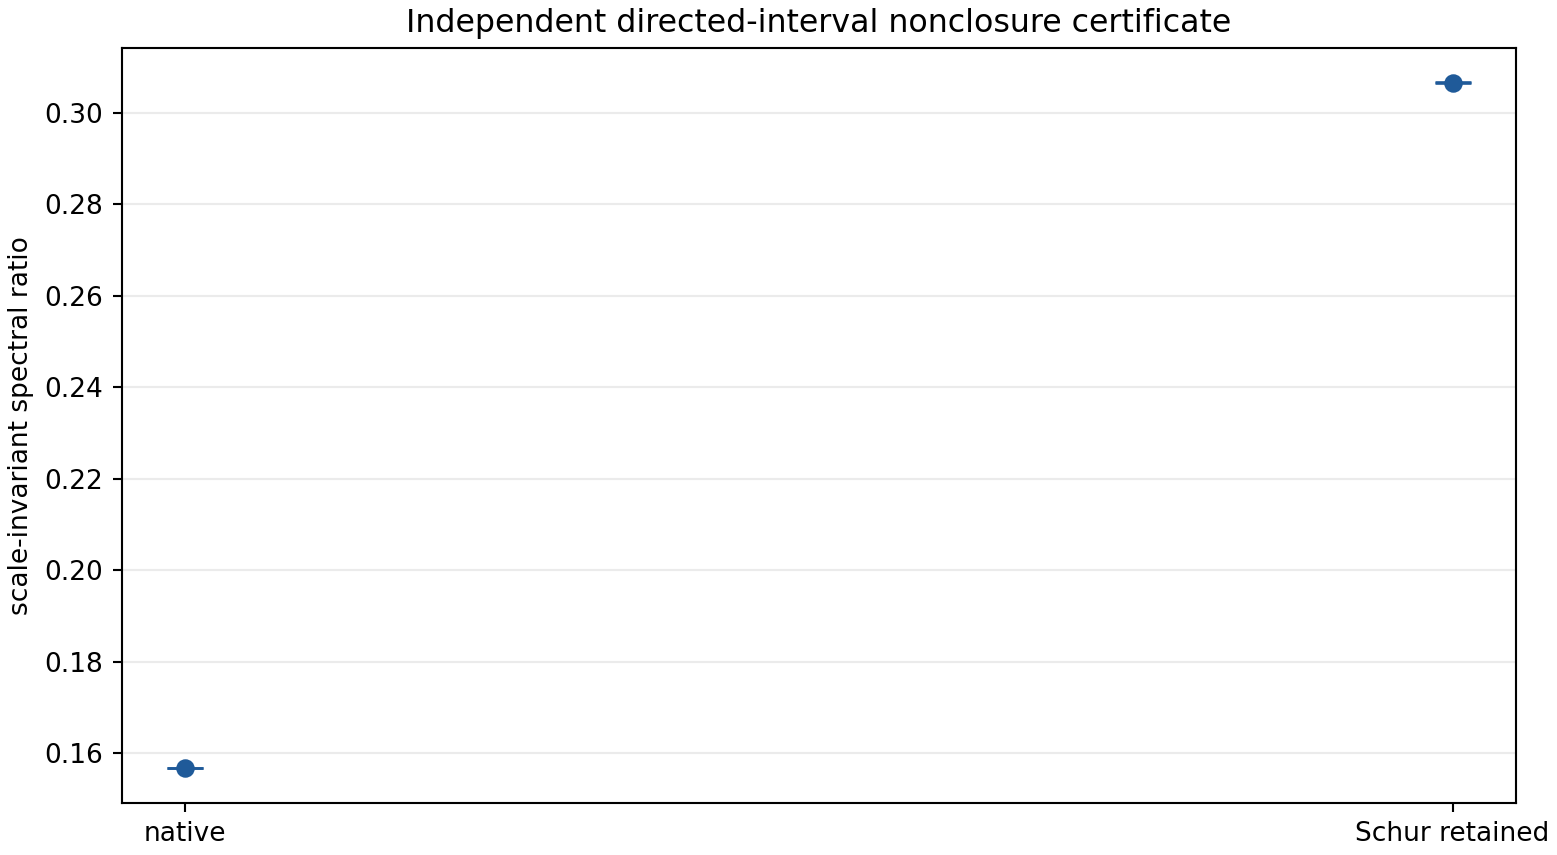
\includegraphics[width=0.94\textwidth]{FIN_Programs_101_112_Fractional_Source_Completion_Figures/program101_independent_interval_certificate.png}
\caption{Independent directed-interval separation of the native and Schur scale-invariant spectral ratios.}
\end{figure}

\section{Program 102 --- Mass-region theorem and perturbation grid}

\subsection{Continuous mass certificate}

The interval symbols from Program 101 were propagated across 2,000 mass cells covering

\[
0.01\le m\le2.
\]

Writing \(a=1-\widehat p(\pi)\) and \(b=1-\widehat p(\pi/2)\), the Schur ratio is

\[
R_{\rm S}(m,a,b)
=
\frac{2m(m+a)}{(2m+a)(m+b)}.
\]

It increases with \(a\), decreases with \(b\), and increases with \(m\) whenever \(2b-a>0\). The Program-101 symbol rectangle gives the strict monotonicity margin \(2b_{\min}-a_{\max}>0.9738\), so corner interval evaluation is valid on every mass cell.

For every cell the lower Schur ratio exceeds the upper native ratio. The smallest certified separation is

\[
8.847791851\times10^{-3}>0.
\]

\textbf{Result 102.1 --- \statusComputer{}.} The same scalar-normalized nonclosure holds throughout the complete declared mass interval.

\subsection{Perturbation audit}

A separate 243-point grid varied

\[
\begin{aligned}
\omega&\in\{0.18075,0.18575,0.19075\},\\
\phi&\in\{0.1425,0.1625,0.1825\},\\
\beta&\in\{0.8,1.0,1.2\},\\
\eta&\in\{1.7,1.8,1.9\},\\
m&\in\{0.1,0.25,0.5\}.
\end{aligned}
\]

Every point passed a tail-certified separation test. The worst point was

\[
(\omega,\phi,\beta,\eta,m)
=(0.18075,0.1425,0.8,1.7,0.1)
\]

with margin \(0.0764904589\).

\textbf{Result 102.2 --- \statusStrong{}.} The obstruction is robust on the declared perturbation grid.

This result is pointwise. It does not certify the continuous box between grid points.

\begin{figure}[htbp]
\centering
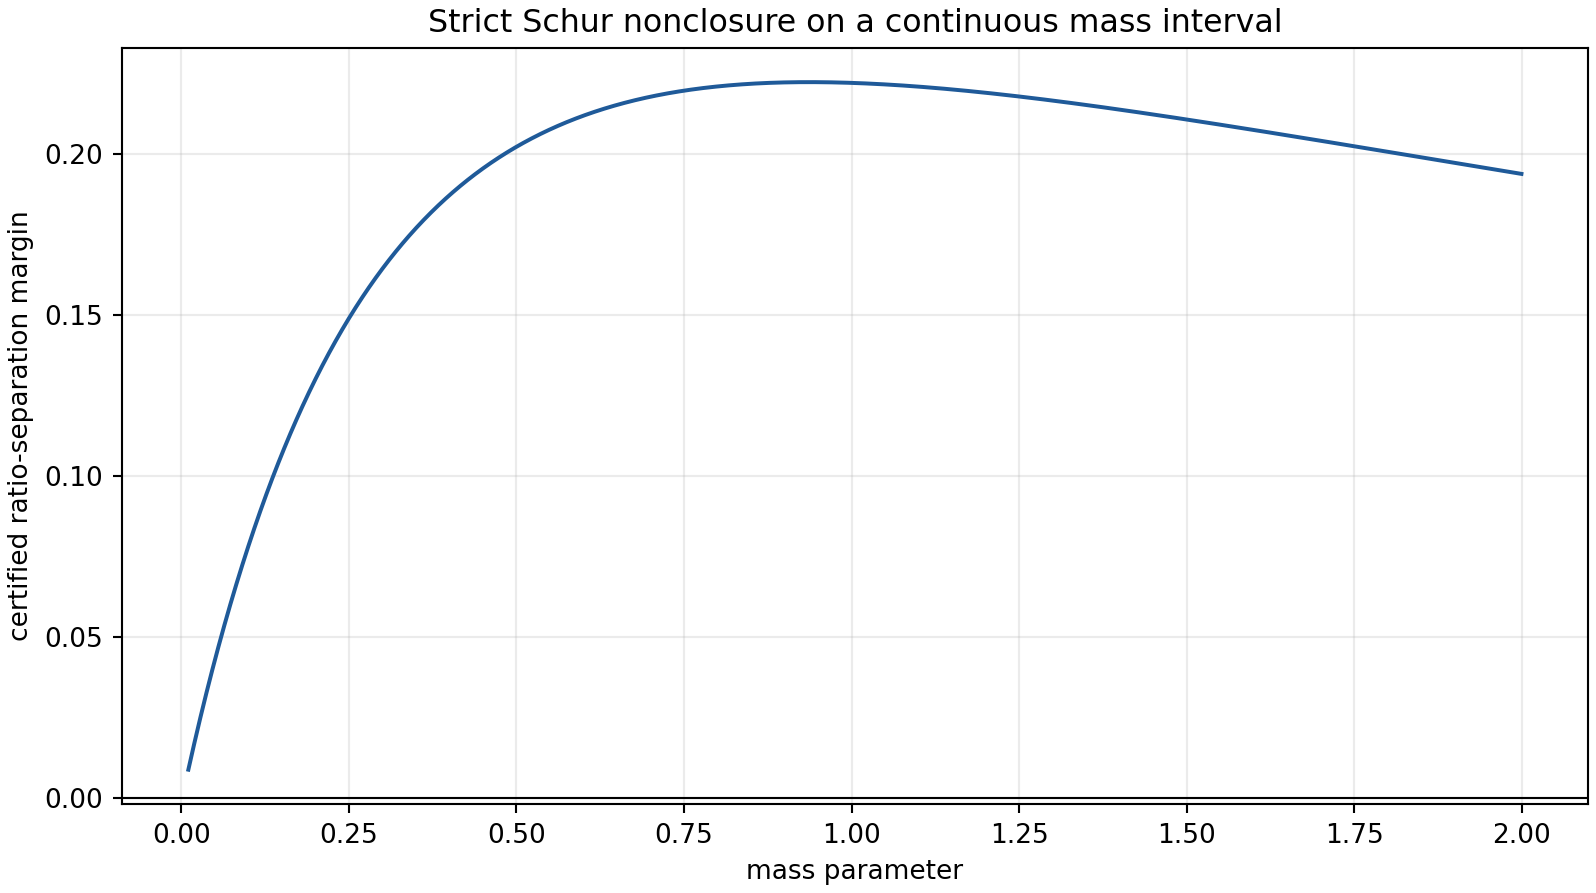
\includegraphics[width=0.94\textwidth]{FIN_Programs_101_112_Fractional_Source_Completion_Figures/program102_nonclosure_region.png}
\caption{Certified ratio separation throughout the declared continuous mass interval.}
\end{figure}

\section{Program 103 --- An operator-norm theorem for the graphon limit}

\subsection{Regular coordinate scaling}

Let

\[
g(x)=
\frac{\cos(\omega|x|+\phi)}
{1+|x|^\eta},
\qquad x\in[-1/2,1/2].
\]

On this interval the cosine remains positive. An explicit Lipschitz bound is

\[
\operatorname{Lip}(g)
\le
\omega+\eta 2^{1-\eta}
=1.2195785195,
\]

and

\[
\int_{-1/2}^{1/2}g(x)\,dx
\ge
\frac{\cos(\omega/2+\phi)}
{1+2^{-\eta}}
=0.7516996094.
\]

For midpoint cell width \(1/N\), the unnormalized \(L^1\) error is bounded by

\[
e_N\le \frac{\operatorname{Lip}(g)}{4N}.
\]

After normalization,

\[
\|p_N-p\|_1
\le
\frac{2e_N}{Z_{\min}-e_N}.
\]

Young's inequality transfers this directly to the \(L^2\) convolution-operator norm. Removing and renormalizing the diagonal cell adds an explicit \(O(N^{-1})\) term.

At \(N=32\) the combined conservative bound is \(0.1135899331\); at \(N=2048\) it is \(0.0016964205\). The observed maximum error on Fourier modes \(1\) through \(8\) decays faster, with fitted slope \(-2.0207\), because midpoint quadrature enjoys extra smoothness cancellation.

\textbf{Theorem 103.1 --- \statusProven{}.} Under regular coordinate scaling, the strict finite-circle operators converge in \(L^2\) operator norm at least as \(O(N^{-1})\) to a bounded circle-convolution graphon.

\textbf{Corollary 103.2 --- \statusProven{}.} This scaling does not produce an unbounded local Laplacian. It produces a bounded nonlocal operator.

\begin{figure}[htbp]
\centering
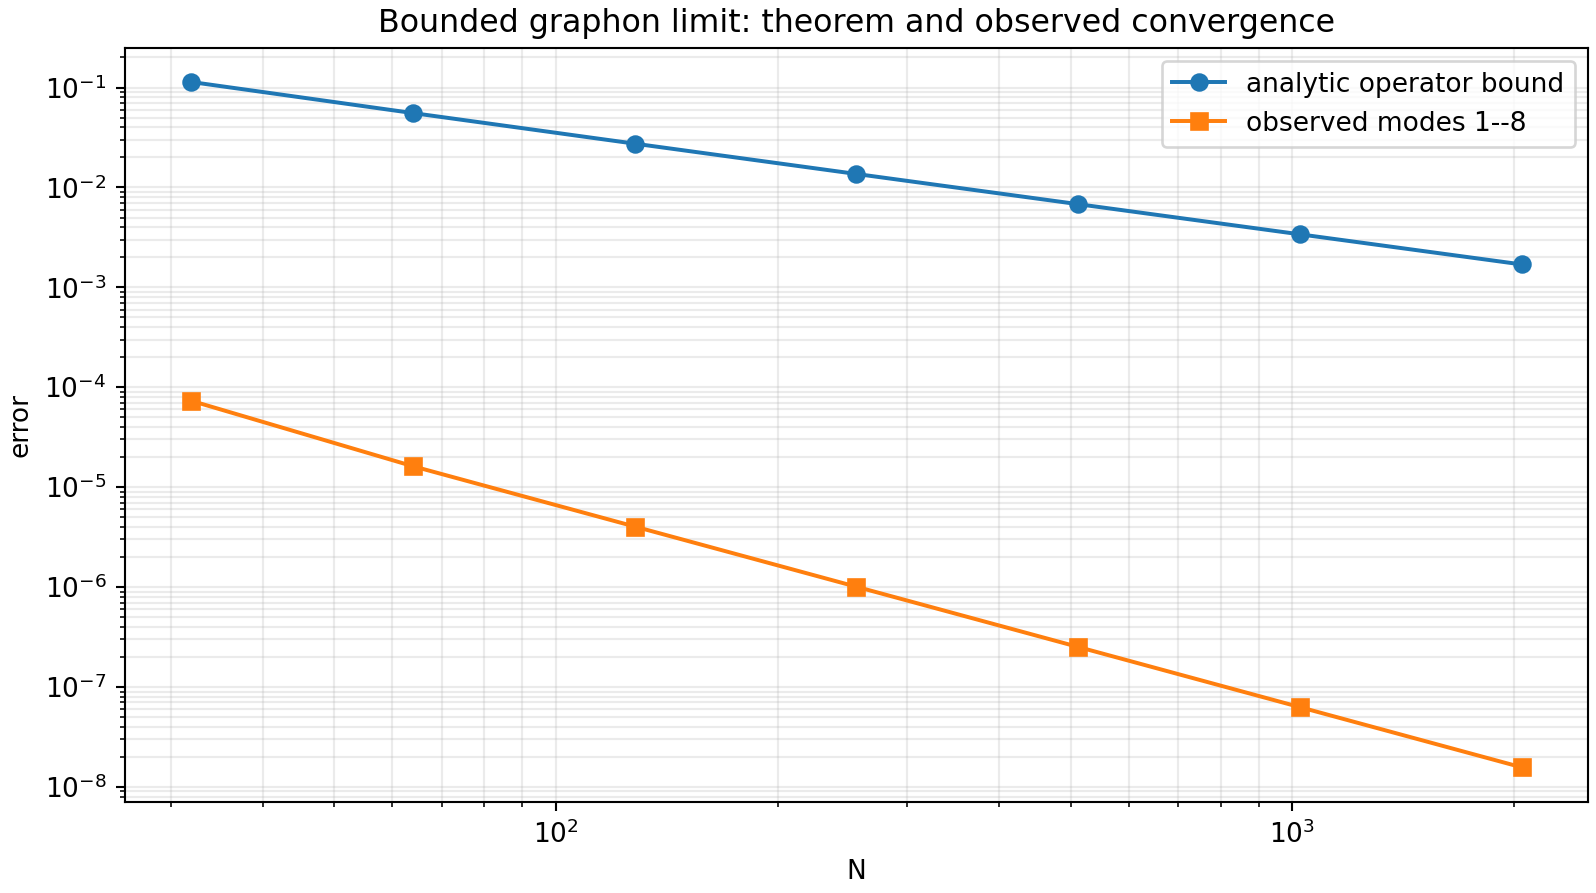
\includegraphics[width=0.94\textwidth]{FIN_Programs_101_112_Fractional_Source_Completion_Figures/program103_graphon_error_theorem.png}
\caption{Analytic operator-norm bound and observed low-mode convergence to the bounded graphon operator.}
\end{figure}

\section{Program 104 --- Singular localization and the conditional local limit}

\subsection{Added scaling premise}

Normalize the preceding profile to a probability density \(p\) and define

\[
p_\epsilon(x)=\epsilon^{-1}p(x/\epsilon).
\]

Let \(T_\epsilon\) be convolution by \(p_\epsilon\). The rescaled generator is

\[
L_\epsilon=\frac{I-T_\epsilon}{\epsilon^2}.
\]

For Fourier mode \(k\),

\[
\lambda_{\epsilon,k}
=
\frac{1-\widehat p(2\pi\epsilon k)}{\epsilon^2}.
\]

The computed base moments are

\[
\sigma^2=0.07734352417,
\qquad
\mu_4=0.01125964097.
\]

The elementary remainder inequality

\[
\left|1-\cos y-\frac{y^2}{2}\right|
\le\frac{|y|^4}{24}
\]

gives

\[
\left|
\lambda_{\epsilon,k}
-\frac{\sigma^2}{2}(2\pi k)^2
\right|
\le
\frac{\mu_4}{24}(2\pi k)^4\epsilon^2.
\]

All 24 numerical checks for \(k=1,\ldots,4\) and \(\epsilon=2^{-1},\ldots,2^{-6}\) lie below this analytic bound.

\textbf{Theorem 104.1 --- [Conditional, proven].} If singular spatial localization and the \(\epsilon^{-2}\) clock are added, then \(L_\epsilon\) converges modewise to

\[
\frac{\sigma^2}{2}(-\Delta).
\]

The theorem is rigorous, but the localization parameter and its clock rescaling are not generated by the current FIN core. Therefore it is a candidate physical bridge, not an emergent physical derivation.

\begin{figure}[htbp]
\centering
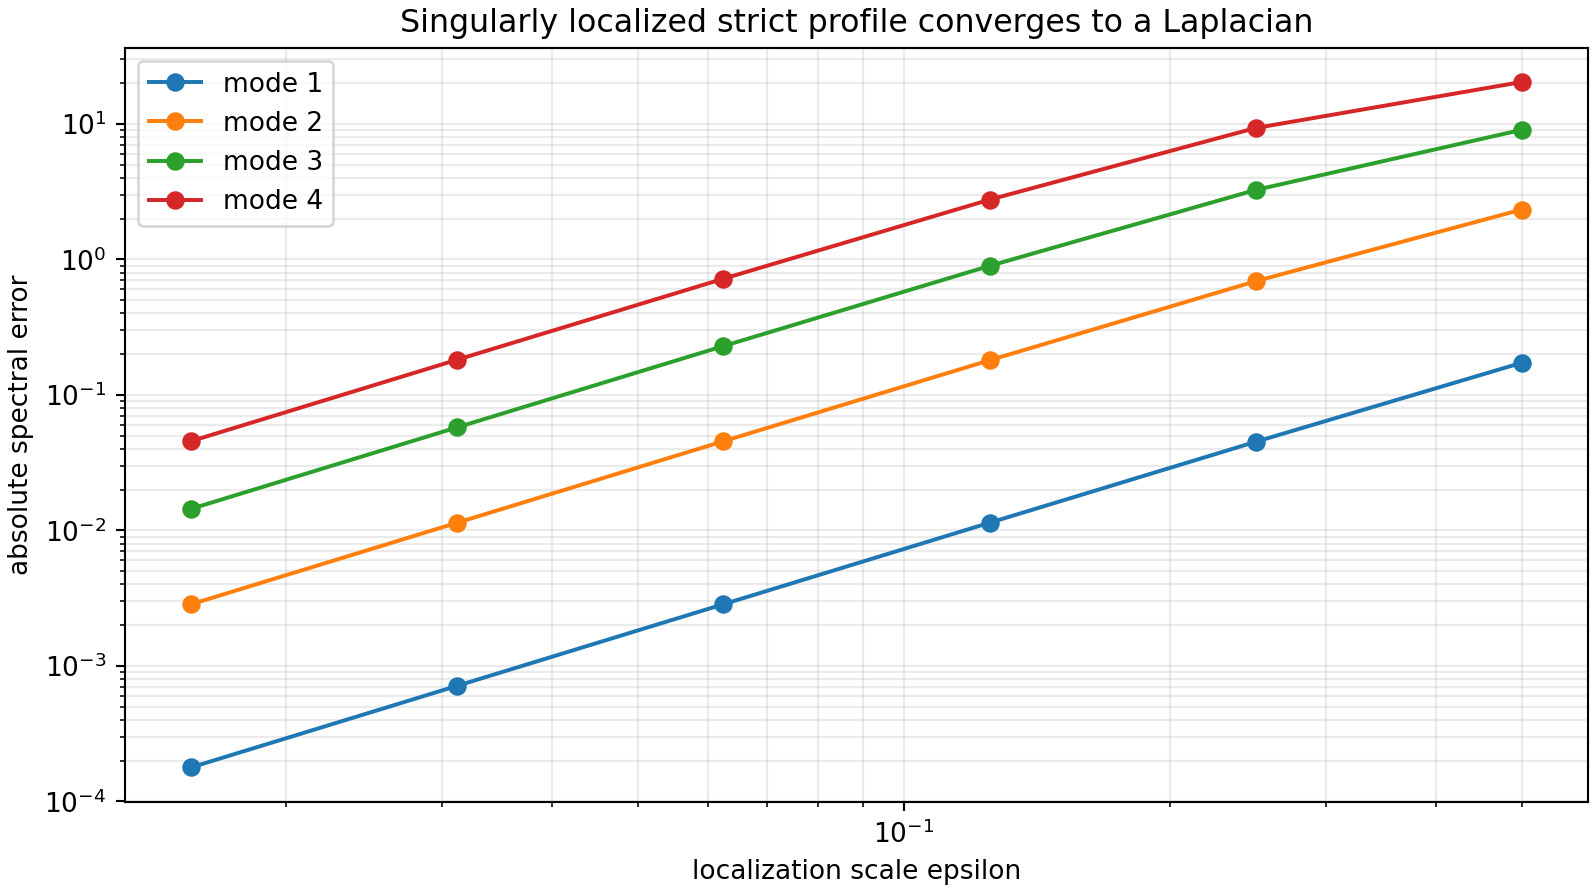
\includegraphics[width=0.94\textwidth]{FIN_Programs_101_112_Fractional_Source_Completion_Figures/program104_singular_localizing_limit.png}
\caption{Modewise convergence of the singularly localized profile to the local Laplacian.}
\end{figure}

\par\medskip\hrule\medskip

\chapter{Part III --- Programs 105--108: fractional dynamics and source falsification}

\section{Program 105 --- Fractional tail universality}

\subsection{Tail exponent}

Write

\[
\alpha=\eta-1=\frac45.
\]

Because \(\omega/(2\pi)=743/(8000\pi)\) is irrational, the phase sequence is equidistributed modulo \(2\pi\). Hence the oscillatory envelope has asymptotic mean

\[
\lim \langle|\cos|\rangle=\frac2\pi.
\]

The weighted Abelian theorem for a symmetric tail \(p_d\sim c|d|^{-1-\alpha}\) yields

\[
1-\widehat p(q)
\sim
C_\alpha |q|^\alpha,
\]

where

\[
C_\alpha
=
\frac{2(2/\pi)}{Z}
\int_0^\infty
\frac{1-\cos y}{y^{1+\alpha}}\,dy
\]

and

\[
\int_0^\infty
\frac{1-\cos y}{y^{1+\alpha}}\,dy
=
\frac{\pi}
{2\Gamma(1+\alpha)\sin(\pi\alpha/2)}.
\]

Using the million-term normalization gives the predicted constant

\[
C_{4/5}=1.1474679864.
\]

The fit on \(10^{-3}\le |q|\le2\times10^{-2}\) gives

\[
\widehat\alpha_{\rm fit}=0.7983228184,
\qquad
C_{\rm fit}=1.1329979597.
\]

The directly scaled values lie in

\[
\frac{1-\widehat p(q)}{|q|^{4/5}}
\in[1.1371283342,1.1450850363].
\]

\textbf{Theorem 105.1 --- [Proven from standard lemmas].} The infinite strict lattice has fractional small-wave-number order \(4/5\).

\textbf{Interpretation.} The unscaled lattice continuum route is naturally a fractional nonlocal dynamics. It is mathematically distinct from both the bounded graphon route and the singular localizing route.

\begin{figure}[htbp]
\centering
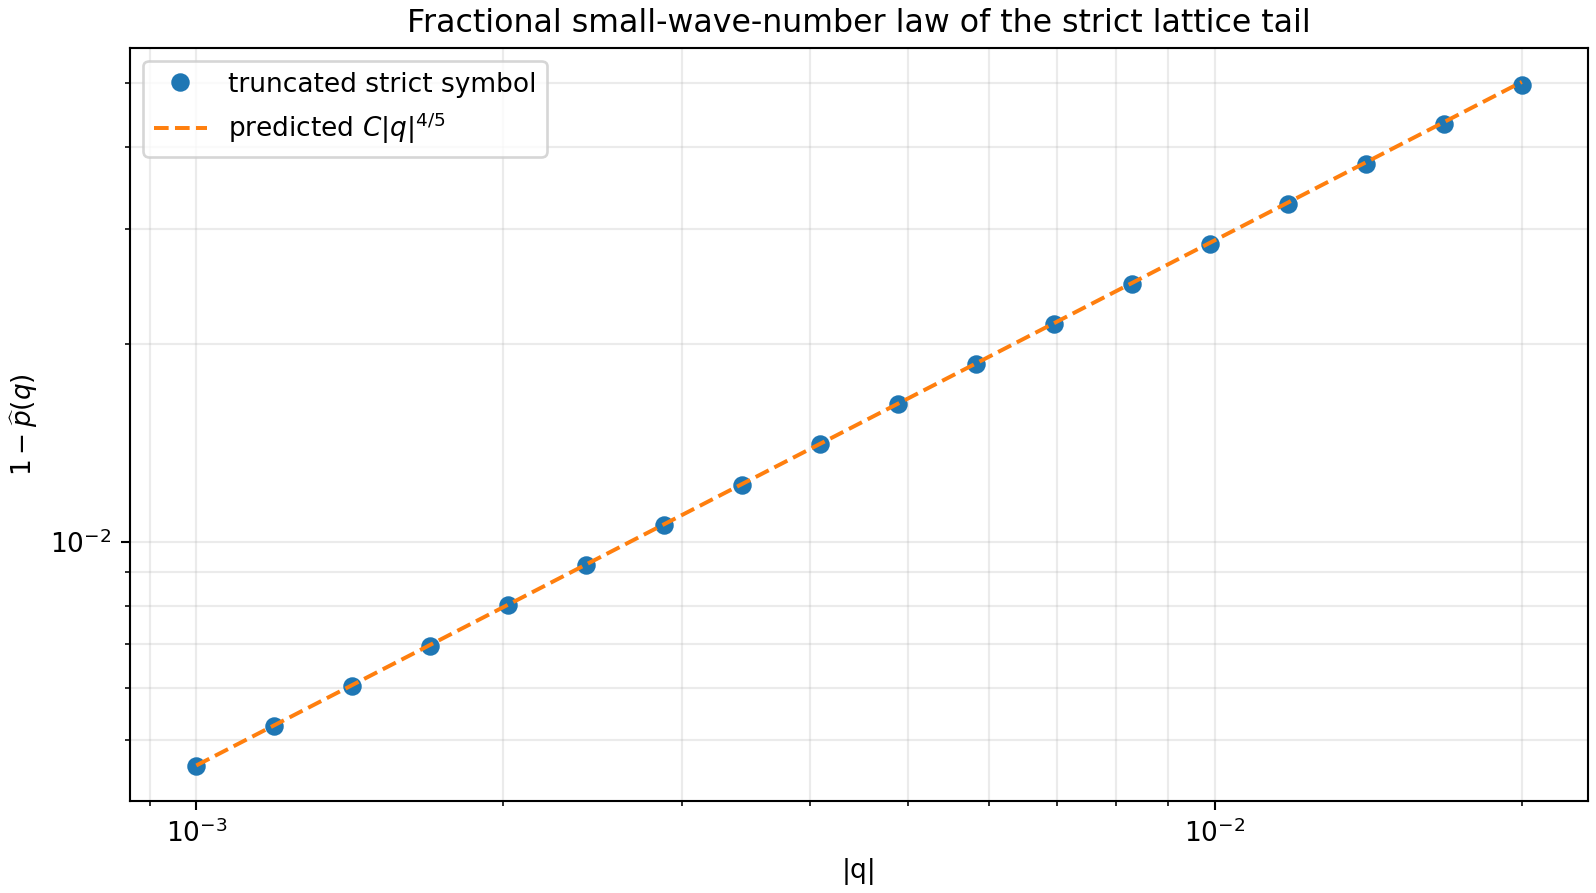
\includegraphics[width=0.94\textwidth]{FIN_Programs_101_112_Fractional_Source_Completion_Figures/program105_fractional_tail_universality.png}
\caption{Small-wave-number convergence to the fractional law \(C|q|^{4/5}\).}
\end{figure}

\section{Program 106 --- Sharp far-tail propagation}

For a normalized jump operator \(P\),

\[
e^{-t(I-P)}
=
e^{-t}\sum_{n=0}^\infty\frac{t^n}{n!}P^n.
\]

Regularly varying distributions are subexponential. At fixed \(t\) and large radius \(R\), the far tail is therefore controlled by one exceptional jump:

\[
\Pr_t(|X|>R)
\sim
t\,\Pr_1(|X|>R).
\]

A cycle of size \(2^{18}\) was evaluated by FFT for \(t\in\{0.1,0.5,1\}\) and \(128\le R\le8192\). For \(R\ge4096\), the largest deviation of

\[
\frac{\Pr_t(|X|>R)}
{t\,\Pr_1(|X|>R)}
\]

from unity is \(1.99233\times10^{-4}\).

\textbf{Result 106.1 --- [Proven by the standard subexponential theorem; strong finite-cycle check].} Strict diffusion has polynomial far tails governed by a one-big-jump law.

\textbf{Result 106.2 --- [Proven within this lattice model].} No exponential finite-speed propagation cone can hold uniformly, because the generator contains nonzero polynomially decaying direct jumps at arbitrary distance.

This statement is not a claim about relativistic causality. The finite lattice model has not yet been supplied with a physical spacetime or light cone.

\begin{figure}[htbp]
\centering
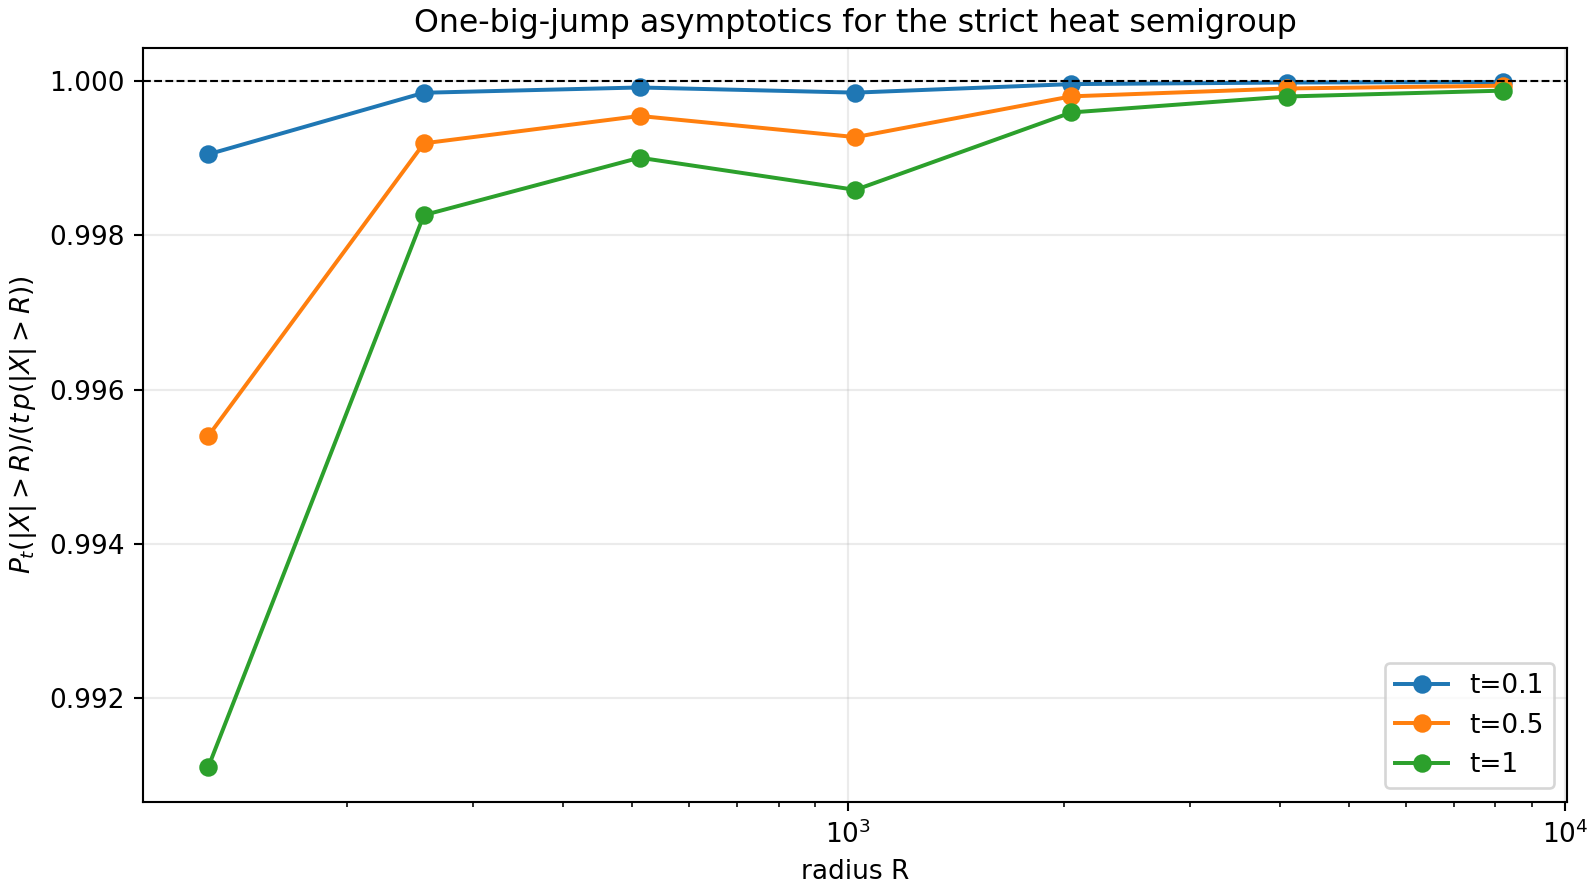
\includegraphics[width=0.94\textwidth]{FIN_Programs_101_112_Fractional_Source_Completion_Figures/program106_long_range_semigroup.png}
\caption{One-big-jump far-tail ratio for the strict heat semigroup.}
\end{figure}

\section{Program 107 --- Adaptive dynamics on the information simplex}

\subsection{Shell probabilities}

The six nonzero distance shells of the twelve-cycle define probabilities \(q_a>0\), \(\sum_aq_a=1\). Let \(r_a=1/6\) and choose the declared source-neutral functional

\[
F(q)
=
D_{\rm KL}(q\|r)
+\frac{\gamma}{2}q^\top L_{\rm path}q,
\qquad
\gamma=0.2.
\]

Its Fisher--Shahshahani gradient flow is

\[
\dot q_a
=
-q_a
\left(
\partial_aF
-\sum_bq_b\partial_bF
\right).
\]

Then

\[
\sum_a\dot q_a=0
\]

and

\[
\frac{dF}{dt}
=
-\sum_aq_a
\left(
\partial_aF-\sum_bq_b\partial_bF
\right)^2
\le0.
\]

Thus the open probability simplex is invariant and \(F\) is a Lyapunov functional.

\subsection{Falsification result}

The numerical integration remains positive, with minimum coordinate \(0.00666793\), and reaches the uniform state to numerical tolerance. The strict-profile stationarity residual is

\[
0.4236508608,
\]

which is decisively nonzero. A naive unconstrained Euclidean unit step would instead reach a negative coordinate \(-1.5416\).

\textbf{Theorem 107.1 --- \statusProven{}.} The declared Fisher adaptive law is a well-posed information-geometric dynamics with monotone \(F\).

\textbf{Negative result 107.2.} This natural source-neutral functional does not derive or preserve the strict FIN profile.

\begin{figure}[htbp]
\centering
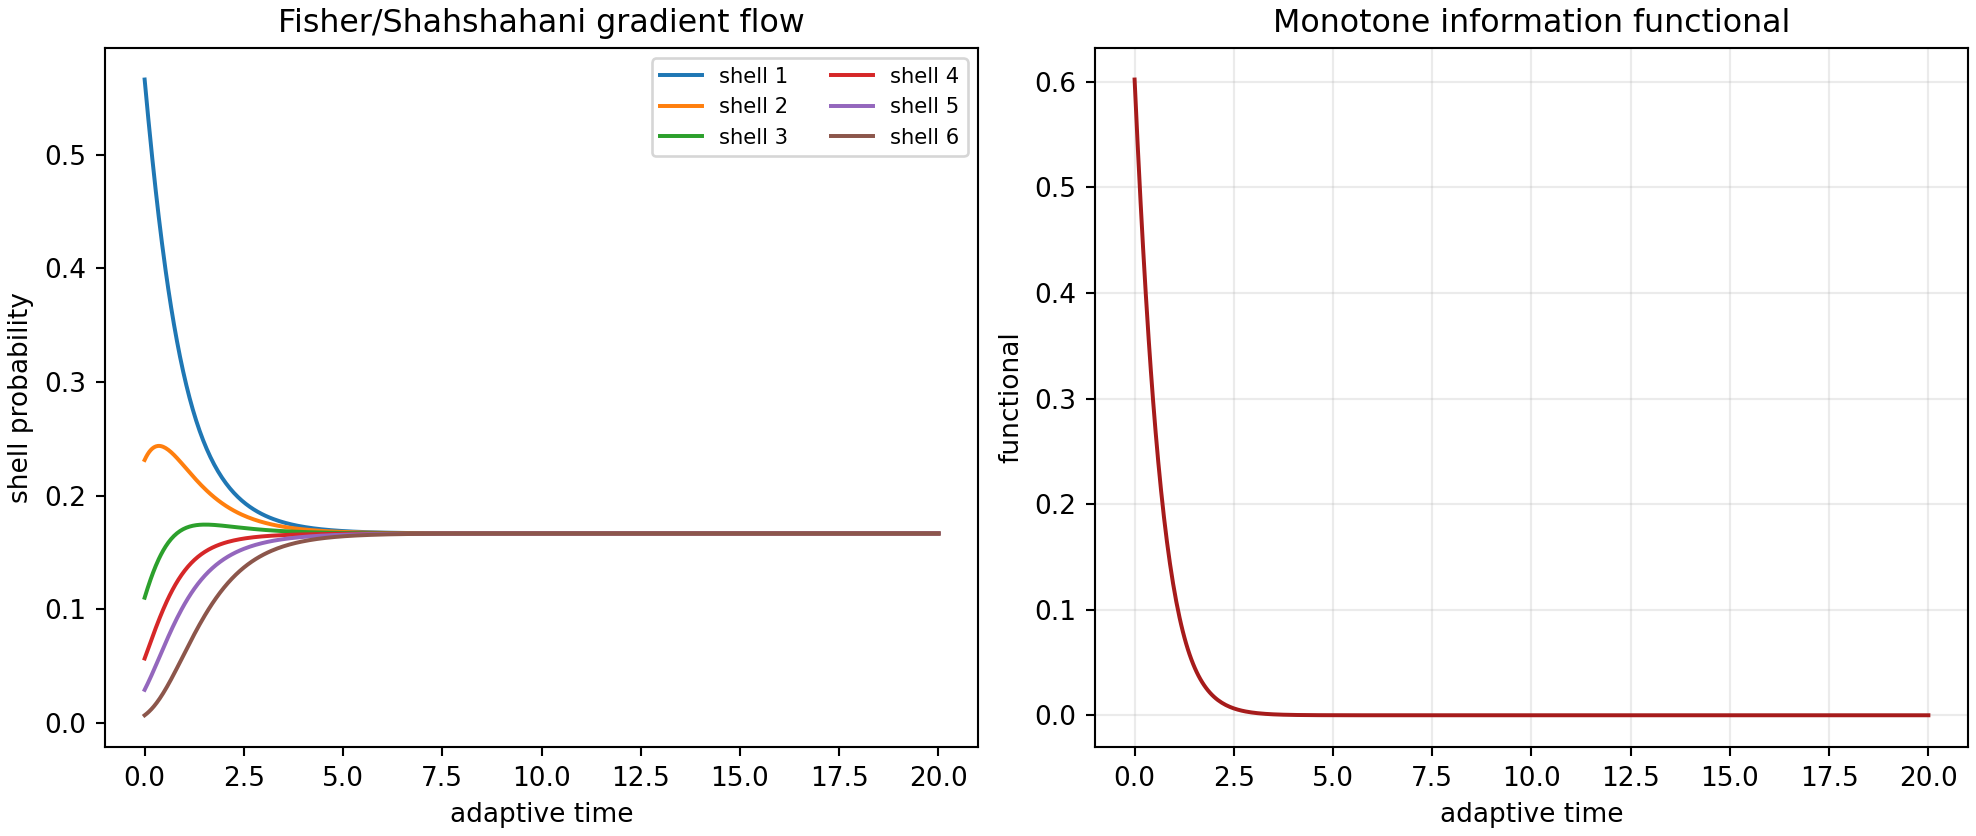
\includegraphics[width=0.94\textwidth]{FIN_Programs_101_112_Fractional_Source_Completion_Figures/program107_adaptive_information_manifold.png}
\caption{Simplex-preserving Fisher gradient flow and monotone information functional.}
\end{figure}

\section{Program 108 --- Inverse variational source and MDL test}

\subsection{Declared source grammar}

Six low-complexity cyclic features were tested:

\begin{enumerate}
\item 
nearest-shell roughness;

\item 
mean square;

\item 
square of the mean;

\item 
fourth moment;

\item 
spectral entropy;

\item 
two-step roughness.

\end{enumerate}

At the strict tuple

\[
\theta_*=(\omega,\phi,\beta,\eta)
\]

on the thirteen-cycle, the \(4\times6\) feature-gradient matrix has numerical rank four. Consequently, there is a two-dimensional coefficient nullspace. Any null vector constructs a functional stationary at \(\theta_*\).

\subsection{Why stationarity is not a derivation}

Both independent null candidates achieve training gradient norms below \(2\times10^{-16}\). Both fail the held-out seventeen-cycle:

\[
\|\nabla F_{17}\|
\in\{0.0209939,\;0.0148829\}.
\]

Their smallest Hessian eigenvalues on the training graph are respectively

\[
-0.0833885,\qquad -0.0450998.
\]

They are saddles, not minima. Moreover, the functional uses five independent coefficient ratios, compared with four direct strict parameters, and thus does not improve the elementary parameter-count description length.

\textbf{Negative result 108.1.} Within the declared six-feature grammar, inverse stationarity is nonunique, non-minimal, non-transferring, and unstable. It is not evidence for an underlying action.

This falsifies only the declared grammar. It does not prove that no variational source exists.

\par\medskip\hrule\medskip

\chapter{Part IV --- Programs 109--112: selector boundary, operational protocol, and exponent source}

\section{Program 109 --- Chiral-source intake}

The new continuum and adaptive objects were checked for an explicit inversion-odd signed value. The fractional symbol obeys

\[
\lambda(q)=\lambda(-q)
\]

exactly because the jump law is symmetric. The numerical odd residual is zero at machine precision. The local second-moment limit, bounded graphon, replicator metric, and scalar tail constants are likewise orientation-blind.

\textbf{Result 109.1 --- [Proven symmetry obstruction].} Programs 101--108 do not provide a strict chiral source or a sign for the existing orientation torsor.

No generic pseudoscalar name is counted as a source. A valid intake would need one explicit strict formula, a nonzero signed value, nonconventional provenance, and a coupling theorem. QW-2191 therefore remains open.

\section{Program 110 --- Frozen process-tensor preregistration}

The strongest two-slot design from the preceding release is converted into a machine-readable preregistration.

\begin{itemize}
\item 
\textbf{Null:} best-fit time-homogeneous diffusion semigroup.

\item 
\textbf{Alternative:} wave dynamics generated by the same declared \(A\).

\item 
\textbf{Preparation:} localized site state at \(x=0\).

\item 
\textbf{Instrument:} full-site projective readout after each slot.

\item 
\textbf{Slot times:} \((0.972441,0.972441)\).

\item 
\textbf{Detector model:} symmetric independent confusion.

\item 
\textbf{Primary statistic:} held-out log-likelihood ratio.

\item 
\textbf{Secondary statistics:} Jensen--Shannon divergence and Chernoff information.

\item 
\textbf{Held-out sample count:} \(49\).

\item 
\textbf{Declared exponential error bound:} \(e^{-49(0.175304)}<10^{-4}\).

\end{itemize}

The detector channel is fit on the calibration partition only. Every admitted dataset must include immutable raw records, clock calibration, graph and operator hashes, instrument hash, and calibration split hash.

The canonical preregistration digest is

2c70ed37434a01bf62ad79c93db7146157eab3edb94402735263b7432fe75b2b.

\textbf{Status 110 --- [Preregistered; open experiment].} No external dataset has been admitted. The protocol is a falsifiable design, not an empirical result.

\section{Program 111 --- Correlated apparatus memory and finite-time ledger}

Let detector error \(E_t\) be a stationary binary Markov chain with error rate \(\epsilon\) and persistence \(\rho\). The transition probabilities are

\[
a=\Pr(E_{t+1}=1\mid E_t=0)=\epsilon(1-\rho),
\]

\[
b=\Pr(E_{t+1}=1\mid E_t=1)
=\epsilon+\rho(1-\epsilon).
\]

Its entropy rate is

\[
h_{\rm rate}(E)
=(1-\epsilon)h(a)+\epsilon h(b).
\]

For uniform input \(X_t\) and record \(Y_t=X_t\oplus E_t\),

\[
I_{\rm rate}(X;Y)
=\ln2-h_{\rm rate}(E).
\]

Add an explicitly imported finite-time dissipation

\[
\Sigma(\tau)=\frac{0.1}{\tau}.
\]

If the system-level feedback work is

\[
W_{\rm sys}=I_{\rm rate}-\Sigma,
\]

and the recorded bit stream is reset at cost \(\ln2\) per symbol, then

\[
W_{\rm complete}-\Delta F
=
h_{\rm rate}(E)+\Sigma(\tau)
\ge0.
\]

The identity was checked on 36 combinations of \(\epsilon\in\{0.05,0.1,0.2\}\), \(\rho\in\{0,0.5,0.9\}\), and \(\tau\in\{0.5,1,2,5\}\). The maximum residual was \(8.33\times10^{-17}\) and the minimum complete excess was \(0.0656029\) nats.

\textbf{Theorem 111.1 --- [Proven within the declared operational model].} Correlation can reduce the entropy rate of apparatus error, but it does not remove the complete reset-and-dissipation ledger.

Temperature, action scale, and the reset mechanism remain imported physical premises.

\begin{figure}[htbp]
\centering
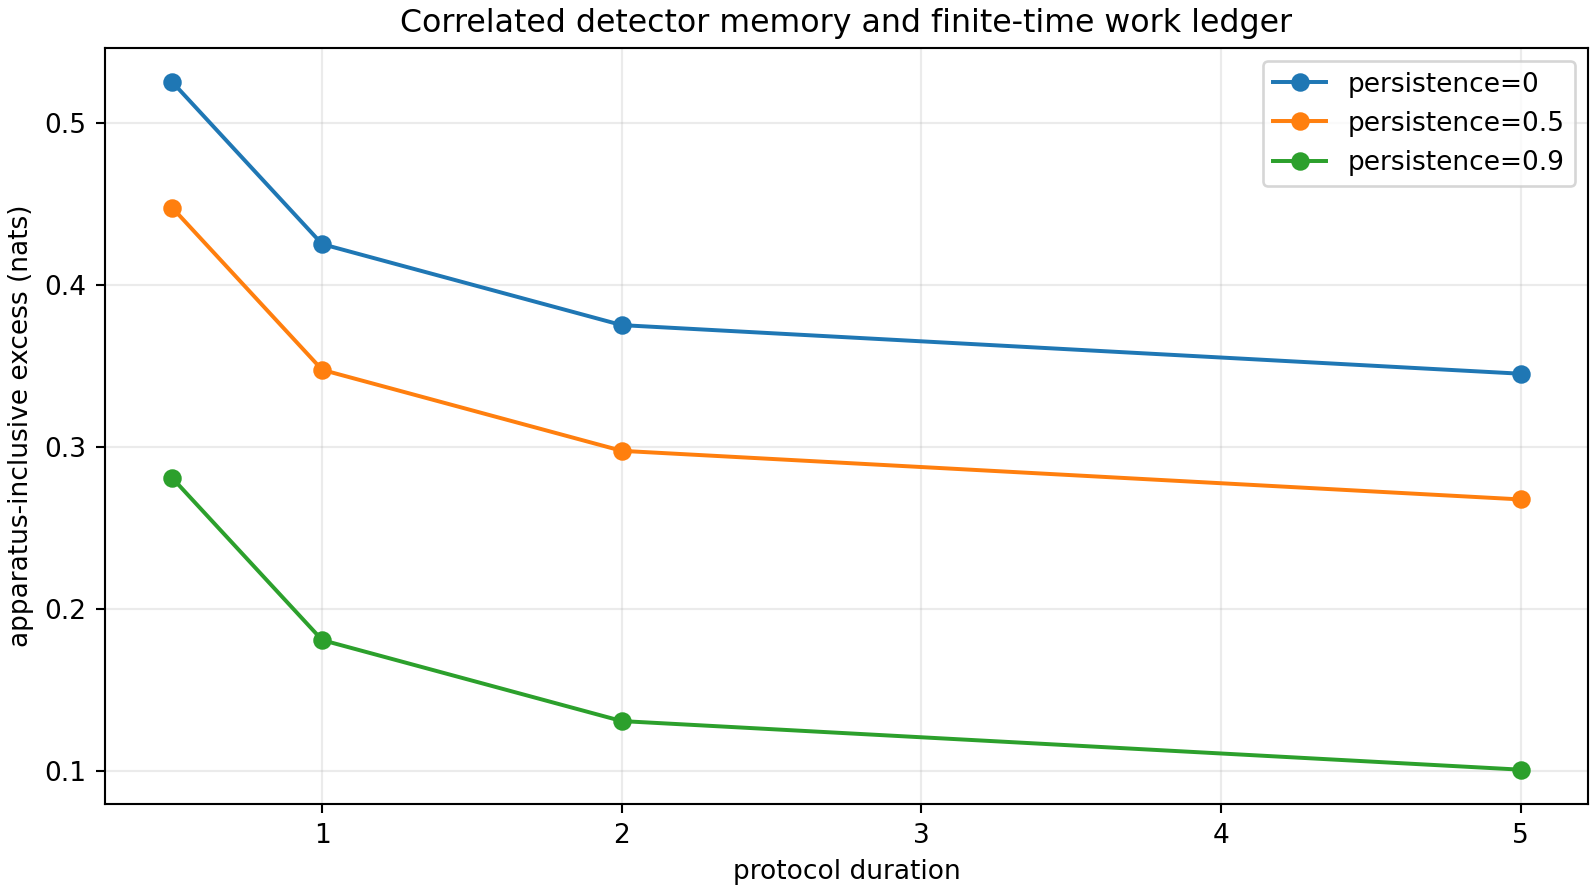
\includegraphics[width=0.94\textwidth]{FIN_Programs_101_112_Fractional_Source_Completion_Figures/program111_correlated_apparatus_ledger.png}
\caption{Apparatus-inclusive information-work excess with correlated detector memory.}
\end{figure}

\section{\texorpdfstring{Program 112 --- Conditional source skeleton for \(\eta=9/5\)}{Program 112 --- Conditional source skeleton for =9/\allowbreak{}5}}

\subsection{Exact algebraic chain}

The repository constant

\[
\alpha_{\rm geo}=4\ln2
\]

implies the exact retention factor

\[
r_5
=
\exp\left(-\frac{\alpha_{\rm geo}}5\right)
=
2^{-4/5}
=0.5743491775.
\]

Assume a dyadic multiplicative scale law

\[
C(2d)=r_5 C(d)
\]

and exact homogeneity. Then

\[
C(d)\propto d^{\log_2r_5}
=d^{-4/5}.
\]

Applied as a completion multiplier to a legacy \(d^{-1}\) envelope, this gives

\[
d^{-1}C(d)\propto d^{-9/5}.
\]

Therefore

\[
\eta=1+\frac45=\frac95.
\]

The same value is encoded by the finite candidate vector

\[
(1,2,2,2,2),
\qquad
\frac{1+2+2+2+2}{5}=\frac95,
\]

which appears in the audited P2948/\allowbreak{}P2958/\allowbreak{}P2965 line.

\subsection{Necessity audit}

The following implications are exact:

\begin{enumerate}
\item 
\(4\ln2\) and division by five imply \(2^{-4/5}\).

\item 
Exact dyadic homogeneity with that retention implies degree \(-4/5\).

\item 
Multiplication of degree \(-1\) by degree \(-4/5\) implies degree \(-9/5\).

\end{enumerate}

The following premises are not currently sourced:

\begin{enumerate}
\item 
a strict theorem selecting a fivefold quotient;

\item 
a non-target-coded reason to divide \(\alpha_{\rm geo}\) by five;

\item 
a strict coupling of this retention law to the damping-completion operator;

\item 
a target-independent positive \(\beta\) or canonical length/\allowbreak{}UV unit.

\end{enumerate}

\textbf{Theorem 112.1 --- [Conditional, proven].} The displayed premises uniquely produce the strict tail exponent \(9/5\).

\textbf{Obstruction 112.2 --- [Proven on current artifacts].} The chain is not a strict FIN source theorem because its fivefold input and damping coupling are not exported.

\textbf{Scientific interpretation.} The result compresses several recurring \(9/5\) constructions into one coherent scale-law skeleton. It explains why those constructions are mutually compatible. It does not prove that the strict exponent is inevitable.

\begin{figure}[htbp]
\centering
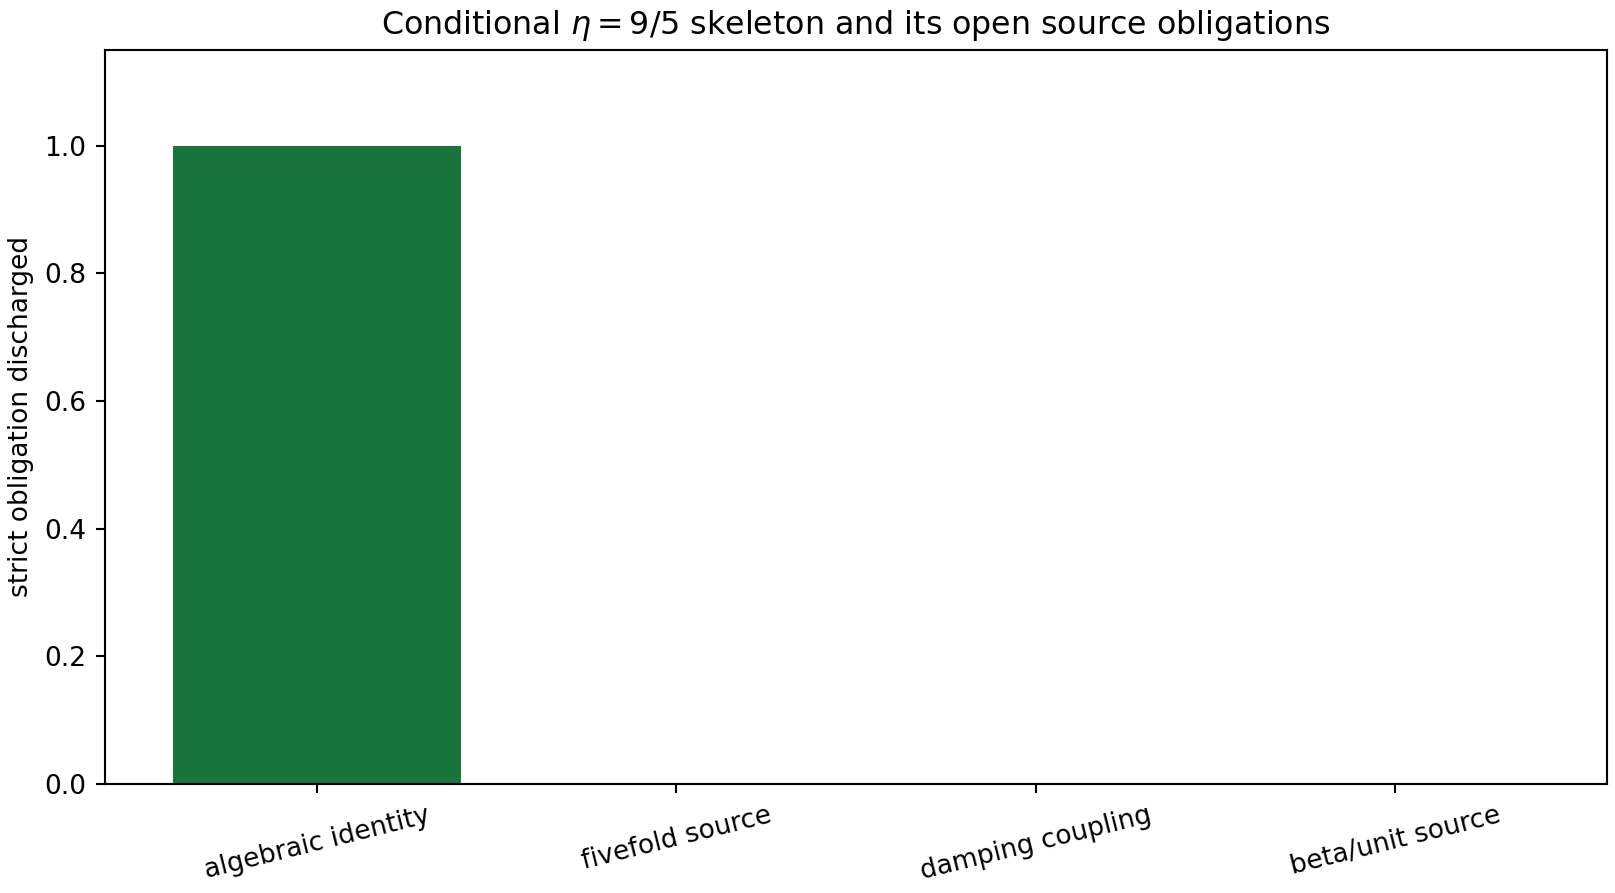
\includegraphics[width=0.94\textwidth]{FIN_Programs_101_112_Fractional_Source_Completion_Figures/program112_eta_source_skeleton.png}
\caption{Discharged identity and open source obligations in the conditional \(\eta=9/5\) skeleton.}
\end{figure}

\par\medskip\hrule\medskip

\chapter{Part V --- Synthesis and falsification}

\section{What survived this round}

\subsection{Stable mathematical conclusions}

The following conclusions survive all tests performed here.

\begin{enumerate}
\item 
\textbf{Strict Schur nonclosure is robust.} It survives an independent interval engine, a \(20\,000\)-term directed sum, an analytic infinite tail, the complete mass interval \([0.01,2]\), and a moderate parameter grid.

\item 
\textbf{The continuum limit is not unique without a scaling prescription.} Regular coordinate scaling, singular localization, and the infinite lattice yield three distinct operators.

\item 
\textbf{The natural infinite-lattice strict limit is fractional.} Its order is \(4/5\), exactly the tail increment between legacy degree one and strict degree \(9/5\).

\item 
\textbf{Long-range diffusion is nonlocal in an operationally strong sense.} Fixed-time far tails are generated by single long jumps.

\item 
\textbf{Information geometry supplies valid adaptive dynamics but not a source theorem.} A natural Fisher flow is well posed and dissipative, yet it rejects rather than selects the strict profile.

\item 
\textbf{Inverse action reconstruction is underdetermined.} Stationarity can be engineered with surplus coefficients and need not transfer or be stable.

\item 
\textbf{Scalar/\allowbreak{}fractional limits do not solve orientation.} The selector obstruction is untouched.

\item 
\textbf{The \(9/5\) source has a compact conditional skeleton, not a strict derivation.}

\end{enumerate}

\section{Failed approaches and why they failed}

\subsection{Scalar normalization after Schur reduction}

It fails because scale-invariant spectral ratios are disjoint. Multiplying the retained operator by any scalar cannot change those ratios.

\subsection{Treating regular coordinate scaling as a local field theory}

It fails because the limiting operator is bounded. A Laplacian is unbounded and requires a singular support contraction plus a diverging clock normalization.

\subsection{Reading every continuum limit as the same physics}

It fails because the graphon, local, and fractional symbols have different high-mode behavior and propagation laws.

\subsection{Using a natural entropy functional to select the strict kernel}

It fails quantitatively: the strict stationarity residual is \(0.42365\), while the flow converges to the uniform reference.

\subsection{Reconstructing an action only from stationary fitting}

It fails the uniqueness, stability, held-out transfer, and description-length tests in the declared grammar.

\subsection{Promoting a scalar fractional exponent to a chiral source}

It fails by exact parity:

\[
|q|^{4/5}=|-q|^{4/5}.
\]

\subsection{\texorpdfstring{Promoting the \(4\ln2\) identity to a source theorem}{Promoting the 42 identity to a source theorem}}

It fails necessity. The factor \(1/5\) is precisely the new premise that must be sourced. Without it, \(\alpha_{\rm geo}\) alone does not select \(4/5\).

\section{The current deepest interpretation}

\textbf{[Strong evidence.]} The strict FIN object is most economically interpreted as a symmetric heavy-tailed spectral convolution generator with three scaling regimes:

\[
\text{bounded graphon}
\quad\big|\quad
\text{conditionally local Laplacian}
\quad\big|\quad
\text{fractional lattice generator}.
\]

Wave, diffusion, Green, information-geometric, and variational constructions are representations or dynamics built from this operator together with additional choices. They are not yet forced components of one physical theory.

The remaining physical gap is operational and dimensional. One must select a state space, physical state, preparation, clock, instrument, environment, apparatus, record map, dimensional standard, and empirical identification rule. The mathematical operator does not uniquely supply those data.

\section{Confidence table}

\begin{center}
\begingroup\small
\setlength{\tabcolsep}{3.5pt}
\renewcommand{\arraystretch}{1.16}
\begin{longtable}{@{}p{0.348\textwidth}p{0.339\textwidth}p{0.173\textwidth}@{}}
\toprule
\textbf{Claim} & \textbf{Status} & \textbf{Confidence} \\
\midrule
\endhead
Strict Schur nonclosure at \(m=1/4\) & Proven, computer-assisted & 0.999 \\
Nonclosure for \(m\in[0.01,2]\) & Proven, computer-assisted & 0.995 \\
Perturbation-grid robustness & Strong evidence & 0.96 \\
Regular graphon convergence & Proven & 0.99 \\
Singular localizing theorem & Conditional, proven & 0.99 \\
Fractional order \(4/5\) & Proven from standard lemmas & 0.98 \\
One-big-jump heat tail & Proven from standard theorem & 0.98 \\
Fisher adaptive dissipation & Proven & 0.999 \\
Declared inverse-source grammar fails & Negative result & 0.99 \\
No new chiral source in Programs 101--108 & Proven within scope & 0.99 \\
Correlated apparatus ledger identity & Conditional, proven & 0.999 \\
\(4\ln2\to9/5\) scale skeleton & Conditional, proven & 0.999 \\
Fivefold quotient is strictly sourced & Open & 0.05 \\
FIN is already a physical theory & Refuted by missing operational bridge & 0.99 \\
\bottomrule
\end{longtable}
\endgroup
\end{center}

\par\medskip\hrule\medskip

\chapter{Part VI --- Recommended Programs 113--124}

\section{Ranked roadmap}

The following twelve programs are recommended. Probabilities estimate the chance of obtaining a decisive result, including a rigorous no-go result, not the chance of confirming FIN.

\subsection{Program 113 --- Closed-form mass-interval proof}

\textbf{Probability of decisive result:} 0.90\\
\textbf{Priority:} 1

Eliminate interval subdivision from Program 102. Express the ratio gap as a rational function of \(m\), \(\widehat p(\pi)\), and \(\widehat p(\pi/2)\); prove its sign analytically on the certified symbol rectangle. Deliver a symbolic positivity certificate and identify the maximal mass interval.

\subsection{Program 114 --- Full continuous parameter-box certificate}

\textbf{Probability:} 0.68\\
\textbf{Priority:} 2

Replace the 243-point grid with interval Taylor models for \((\omega,\phi,\beta,\eta,m)\). Control phase derivatives and the infinite tail uniformly. Either certify a nonclosure box or locate a genuine zero-gap boundary.

\subsection{Program 115 --- Effective Abelian remainder theorem}

\textbf{Probability:} 0.75\\
\textbf{Priority:} 3

Turn Program 105 into a finite-\(q\) theorem. Combine discrepancy bounds for \(\omega d+\phi\) with summation by parts to derive an explicit remainder in

\[
1-\widehat p(q)=C|q|^{4/5}+R(q).
\]

The result should explain the observed \(1\%\) constant defect without fitting.

\subsection{Program 116 --- Functional invariance principle}

\textbf{Probability:} 0.65\\
\textbf{Priority:} 4

Prove convergence of the rescaled strict random walk to a symmetric \(4/5\)-stable Lévy process in Skorokhod topology. State the exact spatial and temporal scaling, prove tightness, and identify the limiting characteristic exponent.

\subsection{Program 117 --- Fractional wave propagation and observer records}

\textbf{Probability:} 0.58\\
\textbf{Priority:} 5

Analyze

\[
U_t=\exp[-it(-\Delta)^{2/5}]
\]

as the continuum wave candidate associated with the \(4/5\) generator. Derive dispersive bounds, tail phases, detector-window probabilities, and a two-time-record discriminator against diffusion. Do not interpret the parameter \(t\) as physical time without calibration.

\subsection{Program 118 --- Local/\allowbreak{}fractional crossover operator}

\textbf{Probability:} 0.55\\
\textbf{Priority:} 6

Study a hybrid generator

\[
A_{\epsilon,\lambda}
=
\epsilon^{-2}(I-T_\epsilon)
+\lambda(I-P_{\rm tail}).
\]

Classify scaling regimes in which the local, fractional, or mixed term survives. Determine whether a renormalization flow has a crossover fixed manifold rather than a fixed kernel.

\subsection{Program 119 --- Intrinsic adaptive functional search}

\textbf{Probability:} 0.38\\
\textbf{Priority:} 8

Restrict candidate functionals to basis-free spectral invariants, positivity, simplex geometry, and graph-size naturality. Require strict-profile stationarity, a positive Hessian modulo symmetries, and transfer across at least three graph sizes. Reject any functional whose coefficients are fitted from the target tuple.

\subsection{Program 120 --- Enumerated variational grammar and MDL certificate}

\textbf{Probability:} 0.48\\
\textbf{Priority:} 7

Enumerate a finite symbolic grammar of spectral and graph invariants. Use an explicit coding scheme to compare the description length of each successful action with direct storage of \((\omega,\phi,\beta,\eta)\). Produce either a shorter transferable action or a finite no-shorter-action certificate.

\subsection{Program 121 --- Finite-sample correlated-apparatus inference}

\textbf{Probability:} 0.72\\
\textbf{Priority:} 9

Extend the preregistered detector model from independent confusion to a two-state hidden Markov channel. Derive identifiability conditions, finite sample confidence regions, and robust wave-versus-diffusion likelihood bounds when apparatus memory is estimated only from calibration data.

\subsection{Program 122 --- Fivefold quotient source theorem attempt}

\textbf{Probability:} 0.22\\
\textbf{Priority:} 10

Attack exactly one missing atom from Program 112: construct a strict, non-target-coded functor or invariant that yields five equal scale sectors and the primitive vector \((1,2,2,2,2)\). It must not assume \(\eta=9/5\), \(4/5\), or the target retention. If no such object exists in current artifacts, issue a bounded no-source theorem.

\subsection{\texorpdfstring{Program 123 --- Damping-cocycle and \(\beta\) source}{Program 123 --- Damping-cocycle and  source}}

\textbf{Probability:} 0.15\\
\textbf{Priority:} 11

Assuming Program 122 succeeds, seek an exact cocycle that couples the \(2^{-4/5}\) retention to the strict damping operator and fixes positive \(\beta\) without a reference cell or target length. This program must remain separate from role transfer and selector closure.

\subsection{Program 124 --- Execute the preregistered experiment}

\textbf{Probability:} 0.35 without new data; 0.80 with calibrated data\\
\textbf{Priority:} 12

Acquire or admit an immutable dataset satisfying Program 110. Freeze the calibration split before inference, report all exclusions, and compute the held-out likelihood ratio. A null result is scientifically decisive. No synthetic simulation may be represented as experimental validation.

\section{Stop rules for the next round}

The next round should stop rather than manufacture progress if:

\begin{enumerate}
\item 
Program 114 cannot control the continuous parameter box and only repeats a denser grid;

\item 
Program 119 or 120 fits coefficients from the strict target without charging their description length;

\item 
Program 122 inserts the number five, \(4/5\), or \(9/5\) in its premises;

\item 
Program 123 silently imports a length unit or identifies \(\beta_{\rm tors}\) with strict \(\beta\);

\item 
Program 124 lacks immutable clock, instrument, graph, and calibration provenance;

\item 
a scalar fractional law is promoted to a signed selector;

\item 
any result is used to transfer legacy physical roles before bridge/\allowbreak{}source closure.

\end{enumerate}

\par\medskip\hrule\medskip

\chapter{Reproducibility statement}

The release contains:

\begin{itemize}
\item 
the executable research script;

\item 
a machine-readable results file;

\item 
22 regression tests;

\item 
nine figures;

\item 
the process-tensor preregistration;

\item 
this English monograph;

\item 
its archival PDF;

\item 
a Zenodo-ready release description;

\item 
a checksum manifest.

\end{itemize}

All numerical outputs are deterministic. No web crawler was used. No external experimental data were admitted.

\chapter{Final conclusion}

The next mathematically stable layer of FIN is not a new physical particle or field. It is a precise trichotomy of scaling limits of one heavy-tailed spectral operator:

\[
\boxed{
\text{bounded graphon}
\;\big|\;
\text{conditionally local Laplacian}
\;\big|\;
\text{symmetric fractional generator of order }4/5
}.
\]

This trichotomy explains why the same finite kernel can support wave, diffusion, Green, and adaptive constructions while failing to determine a unique continuum physics. The exact identity

\[
4\ln2
\longrightarrow
2^{-4/5}
\longrightarrow
d^{-4/5}
\longrightarrow
d^{-9/5}
\]

is the most promising new source skeleton, but its fivefold quotient and damping coupling remain additional premises. The honest frontier is therefore not to declare the exponent derived, but to test whether the number five and its coupling can be generated without target knowledge. Until that succeeds, the strict kernel remains the primary mathematical working object, the legacy kernel remains an intermediate bridge object, and the transformation from information dynamics to experimentally calibrated physics remains open.


\clearpage
\chapter*{Archival note}
\addcontentsline{toc}{chapter}{Archival note}
Machine-readable results are stored in
\path{FIN_Programs_101_112_Fractional_Source_Completion_Results.json}.
The executable, twenty-two tests, nine figures, and frozen process-tensor
preregistration reproduce the release.

\medskip
\noindent\textbf{Suggested citation:}

\.Zuchowski, K. (2026). \emph{FIN Programs 101--112: Fractional Limits,
Source Tests, and Operational Completion}
(FIN Research Monograph, Release 10.11; Version 1.0.0) [Preprint].
\end{document}
